\chapter{Identification and Authentication}
\label{chapter:authentication}
\section{Identification}
The identity of an entity shall have the following properties:
\begin{itemize}
    \item Uniqueness
    \item Unchangable Linking
    \item Lifelong validity
    \item No Transferability
\end{itemize}

In order to identify an entity, an \emph{identifier} has to be defined. The
identifier should meet the above criteria and should be able to determine an
identity \textit{within a given context}.

Identifiers have the purpose of both accountability and access control. They
can be applied to both subjects (users, processes, ...) and objects (files,
URLs, ...), humans and machines, and can be temporary or persistent.

For authentication, a separate \textit{proof of identity} is usually required:

\section{Authentication}
Authentication is the process of confirming whether a second party is indeed who
they claim to be, to a specified level of confidence. There are three basic
forms of authentication:

\begin{itemize}
    \item \emph{Something you know} (passwords)
    \item \emph{Something you have} (smart cards)
    \item \emph{Something you are} (biometrics)
\end{itemize}

Combinations of those increase the security
(\emph{Multi-Factor-Authentication}).

\paragraph{Password Authentication} is based on the \textit{something you know}
factor. Examples include unix passwords, PINs or secret code words. They can
also easily be used to authenticate groups, by distributing the password to
every entity in the group. A weakness of passwords is that an attacker can learn
and reuse it. A possible solution are \textit{one-time passwords}.

\paragraph{One-time Passwords} are only used once, an example would be a TAN
list for online banking. They can also be part of a challenge-response-protocol,
where the two parties agree on a secret function beforehand, and authentication
happens by verifying the function response to a challenge.

\paragraph{Hardware Tokens} take a similar approach in generating some kind of
one-time use token, but those are generated by dedicated hardware, shifting the
factor to \textit{something you have}. They might have an additional input such
as a pin, or, as in the case of popular 2FA solutions, the current time. The
\emph{HOTP} (HMAC-based One-Time Password algorithm) generates short time
passwords using a counter (time) and a pre-shared secret key.

\paragraph{Biometric Authentication} has to be differentiated into
\textit{verification} and \textit{recognition}. In verification, the used
specifies its identity, and the system authenticates the used if biometric
verification succeeds. In recognition, the system recognizes the user amongst
multiple known users without further input.

Biometric authentication systems can fail in two ways: \emph{False negative}
means that a user is incorrectly rejected, a \emph{false positive} means that a
user is wrongly accepted. The threshold on accepting a authentication attempt
has to be chosen in a application specific way, depending on which fault is more
acceptable. \Cref{fig:eer} shows the relationship between the
\textit{False Acceptance Rate} and \textit{False Rejection Rate} with a varying
threshold. A measure of the security of the authentication system could be the
\textit{Equal Error Rate}.
\begin{figure}
    \centering
    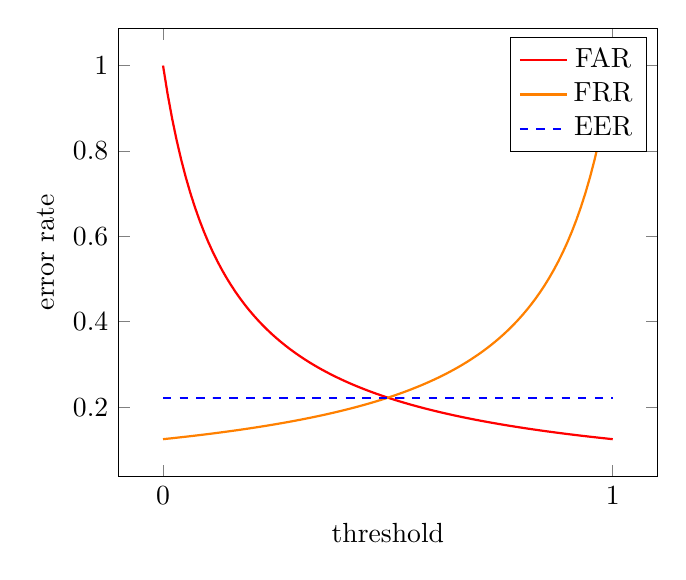
\begin{tikzpicture}
        \begin{axis}[
                xlabel=threshold,
                ylabel=error rate,
                xtick={1,8},
                xticklabels={0,1}
            ]
            \addplot[
                domain=1:8,
                samples=100,
                thick,
                color=red]{1/x};
            \addlegendentry{FAR};
    
            \addplot[
                domain=1:8,
                samples=100,
                thick,
                color=orange]{1/(9-x)};
            \addlegendentry{FRR};
    
            \addplot[
                domain=1:8,
                samples=100,
                dashed,
                thick,
                color=blue]{2/9};
            \addlegendentry{EER};
        \end{axis}
    \end{tikzpicture}
    \caption{\textit{False Acceptance Rate} and \textit{False Rejection Rate}
    for biometric authentication}
    \label{fig:eer}
\end{figure}

\section{Password Security}
Passwords which are short or badly chosen can easily be cracked. Brute-force or
dictionary attacks guess the password either randomly of from a list of known
(pass-)words. Brute-force attacks are easily feasible for passwords up to
\textasciitilde 8 characters in length, useful rules on possible guesses and
dictionary attacks can lead to success for even longer passwords. An advantage
for the attacker is when the attack can be executed \textit{offline}, such as by
stealing the file containing the password hashes. This removes the bottleneck of
the authentication mechanism of the target and allows for distributed attacks.

A common protection measure is to use a \emph{SALT}. A salt is a random value
that gets appended to the password before hashing, and then gets stored
alongside the password hash. While this does not protect a single password
against the mentioned attacks, it prevents reuse of a hash that has already been
calculated. Otherwise, it would be possible to just compare the hashes to known
hashes of popular passwords.

Another consideration is access to the password hashes. While the actual
cryptographic security is only influenced by the hash function, preventing
offline attacks by properly protecting the hashes forces the attacker to execute
much slower online attacks. Those online attacks can be slowed even further by
limiting the number of invalid authentication attempts or introducing an
increasing delay after failed authentication attempts (\textit{back off}), and
by using ``slow'' hash functions. The previously popular measure of password
aging (requiring passwords to be changed after a certain amount of time) is
discouraged, since it promotes the use of weak but easy to remember passwords.

Other attacks focus on the specific implementation of the authentication
mechanism and exploit vulnerabilities that allow login even without actually
obtaining the correct password, or allow changing or resetting passwords even
with insufficient privileges.

\subsection{Time Memory Trade-off}
In attacks on passwords a trade-off between time and memory has to be made, the
two extremes being the brute-force attack and the fully pre-calculated
dictionary/codebook attack.

One possible solution is a \emph{Variable Length Lookup Table}. Those rely on
hash chains: For many initial values, a chain of hashes (length $n_\text{max}$)
each is calculated. Only the initial and end-value are for each chain is then
stored. When a certain hash shall then be cracked, it will be hashed
$n_\text{max}$ times until a chain is found which end-state matches the
calculated hash. Once the chain is found, it can be restored using the stored
initial state which results in a chain containing the to-be-cracked hash and the
password as the state immediately preceding that value.

An improvement to lookup time can be made by making the chains variable length,
and introducing an end criterion, for example a certain number of zero-bits at
the end of the hash (\emph{Distinguished Codepoints}). This reduces the number
of end-lookups significantly.

Duplication arising from hash collisions are addressed by \emph{Rainbow Tables}:
A round-specific reduction function (hash space \textrightarrow password space)
is introduced. So even if a state is already present in a different chain (but
at another round in the chain), the original chain continues separately.

\section{Network Authentication}
\todo[inline]{Authentication: Network Authentication}
